              
% ****** Start of file apssamp.tex ******
%
%   This file is part of the APS files in the REVTeX 4.1 distribution.
%   Version 4.1r of REVTeX, August 2010
%
%   Copyright (c) 2009, 2010 The American Physical Society.
%
%   See the REVTeX 4 README file for restrictions and more information.
%
% TeX'ing this file requires that you have AMS-LaTeX 2.0 installed
% as well as the rest of the prerequisites for REVTeX 4.1
%
% See the REVTeX 4 README file
% It also requires running BibTeX. The commands are as follows:
%
%  1)  latex apssamp.tex
%  2)  bibtex apssamp
%  3)  latex apssamp.tex
%  4)  latex apssamp.tex
%
\documentclass[%
 reprint,
%superscriptaddress,
%groupedaddress,
%unsortedaddress,
%runinaddress,
%frontmatterverbose, 
%preprint,
%showpacs,preprintnumbers,
%nofootinbib,
%nobibnotes,
%bibnotes,
 amsmath,amssymb,
 aps,
%pra,
%prb,
%rmp,
%prstab,
%prstper,
%floatfix,
]{revtex4-1}

\usepackage{graphicx}% Include figure files
\usepackage{dcolumn}% Align table columns on decimal point
\usepackage{bm}% bold math
\usepackage{hyperref}% add hypertext capabilities
%\usepackage[mathlines]{lineno}% Enable numbering of text and display math
%\linenumbers\relax % Commence numbering lines

%\usepackage[showframe,%Uncomment any one of the following lines to test 
%%scale=0.7, marginratio={1:1, 2:3}, ignoreall,% default settings
%%text={7in,10in},centering,
%%margin=1.5in,
%%total={6.5in,8.75in}, top=1.2in, left=0.9in, includefoot,
%%height=10in,a5paper,hmargin={3cm,0.8in},
%]{geometry}
\bibliographystyle{plain}

%\graphicspath{{C:\Users\Nick\Documents\GitHub\FYS2150\lab1}}

\begin{document}

%\preprint{APS/123-QED}

\title{FYS2150 \\
Lab Report: Time and Frequency}% Force line breaks with \\

\author{Nicholas Karlsen}
% \email{nichoka@student.matnat.uio.no}

\date{\today}% It is always \today, today,
             %  but any date may be explicitly specified

\begin{abstract}
The goal for this lab was measuring time, and comparing three methods of doing so, of varying degrees of "sophistication"; an hourglass, a stopwatch and a photodiode.
\end{abstract}

\maketitle

%\tableofcontents

\section{\label{sec:intro}Introduction}
	The lab spanned 6 hours and consisted of measuring the period of a pendulum using three different methods of measurement; an hourglass, a stopwatch and a photodiode connected to a computer. The experiments were performed by myself, and my lab partner Lars K. Skaarseth.
	Before anything else, it is worth to note that the first experiment can largely be disregarded due to an error on our part, more on this in section \ref{subsec:hourglass}.

\section{Theory}
	The theory used in this lab report is almost entirely summed up by the following equations;
	\begin{equation}
		T = 2\pi \sqrt{\frac{L}{g}}
	\end{equation}
	Where $T$ denotes the period a swinging pendulum, $L$ the length of the wire by which the pendulum is suspended and $g$ the downward acceleration on the pendulum due to gravity.
	\begin{equation}
		\vec R = \frac{1}{M} \sum_i m_i \vec r_i
	\end{equation}
	Where $\vec R$ denotes the position of the center of mass of a body of mass $M$ consisting of several smaller bodies of mass $m_i$ with individual center of mass at $r_i$.

	Further detail can be found in "Elementary Mechanics Using Python" \cite{elempy}, or most other books covering introductory mechanics.

\section{Experimental Procedure}
	\subsection{\label{subsec:hourglass}Hourglass}
	\subsection{\label{subsect:stopwatch}Stopwatch}
	\subsection{Photodiode}
\section{Results}
	\subsection{Pendulum \& Hourglass}
	\begin{center} % Pendulum and hourglass
	    \begin{tabular}{| l | l |}
		    \hline
		    Recording no. & Number of oscilations\\ \hline
		    1 & 116 \\ \hline
		    2 & 121 \\ \hline
		    3 & 128 \\ \hline
	    \end{tabular}
	\end{center}

	\subsection{Pendulum \& Stopwatch}
	\begin{center} % Pendulum and stopwatch
	    \begin{tabular}{| p{1.5cm} | p{2cm} | p{2cm} |}
		    \hline
		    Number of periods & Time [sec] & Total time [min:sec] \\ \hline
		    10 & 14.14 & 14.14 \\ \hline
		    20 & 14.31 & 28.53 \\ \hline
		    30 & 14.32 & 42.85 \\ \hline
		    40 & 14.40 & 57.25 \\ \hline
		    50 & 14.29 & 1:11.54 \\ \hline
		    60 & 14.39 & 1:25.93 \\ \hline
		    70 & 14.29 & 1:40.72 \\ \hline
		    80 & 14.34 & 1:54.46 \\ \hline
		    90 & 14.20 & 2:08.76 \\ \hline
		    100 & 14.52 & 2:23.28 \\ \hline
	    \end{tabular}
    \end{center}
    
    \subsection{Pendulum \& Photodiode}

    	\begin{center} % Pendulum and stopwatch
	    \begin{tabular}{| p{1.7cm} | p{1.5cm} | p{1.5cm} | p{1.5cm} | p{1.5cm} | p{1.5cm} |}
		    \hline
		    Experiment no. & Standard deviation of mean period & Mean period & Position of diode & Total measured time [s] & Measuring frequency [KHz] \\ \hline
		    1 & 5.6540e-4 & 1.4421 & Bottom & 120 & 25 \\ \hline
		    2 & 8.8552e-4 & 1.4502 & Bottom & 120 & 200 \\ \hline
		    3 & 0.0483 & 1.5816 & top & 120 & 25 \\ \hline
		    4 & 0.0026 & 1.4922 & Bottom & 120 & 25 \\ \hline
	    \end{tabular}
    \end{center}
    
    \begin{figure}[h!]
    	\center
    	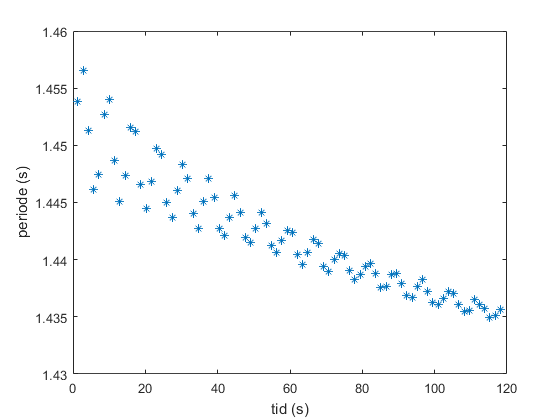
\includegraphics[scale=0.6]{forsok1fig1}
    	\caption{Data from Experiment no. 1 using the photodiode
    	\footnote{Due to bad planning on my part, this figure, and the following all lack figure titles.
    	}}
    \end{figure}

    \begin{figure}[h!]
    	\center
    	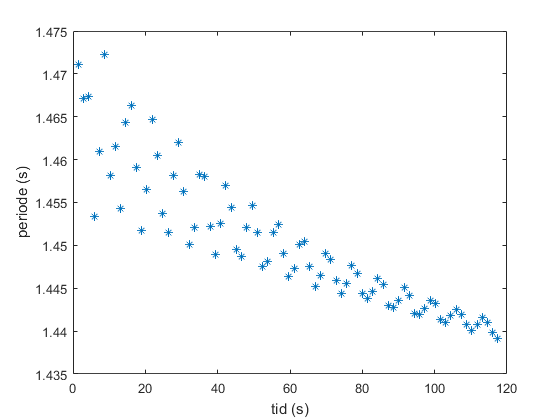
\includegraphics[scale=0.6]{forsok2fig1}
    	\caption{Data from Experiment no. 2 using the photodiode}
    \end{figure}

    \begin{figure}[h!]
    	\center
    	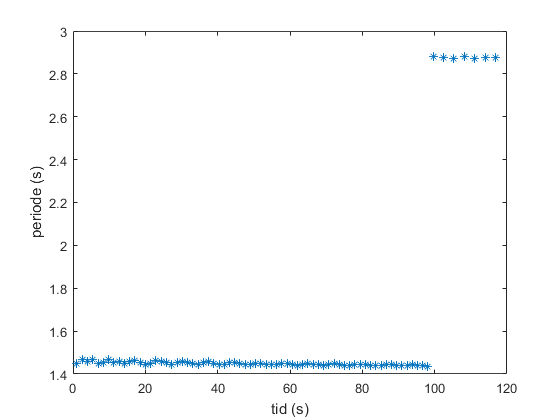
\includegraphics[scale=0.6]{forsok3fig1}
    	\caption{Data from Experiment no. 3 using the photodiode}
    \end{figure}

    \begin{figure}[h!]
    	\center
    	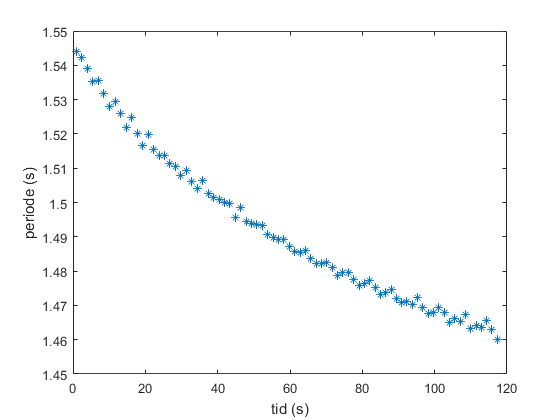
\includegraphics[scale=0.6]{forsok4fig1}
    	\caption{Data from Experiment no. 4 using the photodiode}
    \end{figure}
  	
  	Experimenting experiments Experimenting experiments Experimenting experiments Experimenting experiments Experimenting experiments Experimenting experiments Experimenting experiments Experimenting experiments Experimenting experiments 


\section{Discussion}
	Discussing results Discussing results Discussing results Discussing results Discussing results Discussing results Discussing results Discussing results Discussing results Discussing results Discussing results Discussing results Discussing results Discussing results Discussing results Discussing results Discussing results Discussing results Discussing results Discussing results Discussing results Discussing results Discussing results Discussing results Discussing results Discussing results Discussing results Discussing results Discussing results Discussing results Discussing results Discussing results Discussing results Discussing results Discussing results Discussing results 
\section{Conclusion}
	Concluding conclusions Concluding conclusions Concluding conclusions Concluding conclusions Concluding conclusions Concluding conclusions Concluding conclusions Concluding conclusions Concluding conclusions Concluding conclusions Concluding conclusions Concluding conclusions Concluding conclusions Concluding conclusions 

\bibliography{rapport1_ref}

\end{document}
%
% ****** End of file apssamp.tex ******
              